\documentclass[conference]{IEEEtran}
\usepackage{times}

% numbers option provides compact numerical references in the text.
\usepackage[numbers]{natbib}
\usepackage{multicol}
\usepackage[bookmarks=true]{hyperref}

\usepackage{graphicx} % more modern
%\usepackage{epsfig} % less modern
\usepackage{subfigure}

% For algorithms
\usepackage{algorithm}
\usepackage{algorithmic}
\usepackage{amsmath}
\usepackage{amssymb}
% Include other packages here, before hyperref.
\usepackage{color}
\usepackage{setspace}
\usepackage{wrapfig}
\usepackage{dsfont}

\usepackage[it,small]{caption}


\newcommand{\argmax}{\operatorname{arg\,max}}
\newcommand{\argmin}{\operatorname{arg\,min}}
\newcommand{\todo}[1]{\textcolor{blue}{\textbf{#1}}}
\newtheorem{mydef}{Definition}



\graphicspath{{./images/}}
\usepackage{multirow}
% Some illegal space-saving macros
%  \parskip=5pt
%  \abovedisplayskip 3.0pt plus2pt minus2pt%
% \belowdisplayskip \abovedisplayskip
% \renewcommand{\baselinestretch}{0.97}



\newenvironment{packed_enum}{
\begin{enumerate}
  \setlength{\itemsep}{0pt}
  \setlength{\parskip}{0pt}
  \setlength{\parsep}{0pt}
}
{\end{enumerate}}

\newenvironment{packed_item}{
\begin{itemize}
  \setlength{\itemsep}{0pt}
  \setlength{\parskip}{0pt}
  \setlength{\parsep}{0pt}
}{\end{itemize}}


 \newlength\savedwidth
 \newcommand\whline[1]{\noalign{\global\savedwidth\arrayrulewidth
								\global\arrayrulewidth #1} %
					   \hline
					   \noalign{\global\arrayrulewidth\savedwidth}}
 \renewcommand\multirowsetup{\centering}


\newlength{\sectionReduceTop}
\newlength{\sectionReduceBot}
\newlength{\subsectionReduceTop}
\newlength{\subsectionReduceBot}
\newlength{\abstractReduceTop}
\newlength{\abstractReduceBot}
\newlength{\captionReduceTop}
\newlength{\captionReduceBot}
%\newlength{\nameReduceTop}
\newlength{\subsubsectionReduceTop}
\newlength{\subsubsectionReduceBot}

\newlength{\horSkip}
\newlength{\verSkip}

\newlength{\figureHeight}
\setlength{\figureHeight}{1.7in}

%\newlength{\figureFraction}
\setlength{\horSkip}{-.09in}
\setlength{\verSkip}{-.1in}
%\setlength{\figureFraction}{.195}


%
\setlength{\subsectionReduceTop}{-0.05in}
\setlength{\subsectionReduceBot}{-0.15in}
\setlength{\sectionReduceTop}{-0.07in}
\setlength{\sectionReduceBot}{-0.1in}
\setlength{\subsubsectionReduceTop}{-0.06in}
\setlength{\subsubsectionReduceBot}{-0.05in}
%
%
%\setlength{\figureHeight}{1.5in}
\setlength{\abstractReduceTop}{-0.10in}
\setlength{\abstractReduceBot}{-0.05in}
%
%

%\setlength{\nameReduceTop}{-0.05in}


\setlength{\captionReduceTop}{-0.15in}
\setlength{\captionReduceBot}{-0.15in}



\pdfinfo{
   /Author (Homer Simpson)
   /Title  (Robots: Our new overlords)
   /CreationDate (D:20101201120000)
   /Subject (Robots)
   /Keywords (Robots;Overlords)
}

\usepackage{helvet}
%\renewcommand{\familydefault}{\sfdefault}

\begin{document}


% paper title
\title{Supplementary Material For \\ rCRF: Recursive Belief Estimation over CRFs in RGB-D Activity Videos}

% You will get a Paper-ID when submitting a pdf file to the conference system
%\author{Author Names Omitted for Anonymous Review. Paper-ID 63}
\author{
\authorblockN{Ozan Sener}
\authorblockA{School of Electrical \& Computer Eng. \\ Cornell University}
\and
\authorblockN{Ashutosh Saxena}
\authorblockA{Department of Computer Science \\ Cornell University}
}


\maketitle

\IEEEpeerreviewmaketitle
\section{Recursive Conditional Random Field}
%\vspace{\subsectionReduceTop}
\begin{mydef}
Let $\mathcal{G}^t=(V^t,E^t)$ be set of graphs indexed by the temporal variable $t$ and $\mathbf{y}^t$ is indexed by the vertices of $\mathcal{G}^t$ as $\mathbf{y}^t=(y^t_v)_{v \in V^t}$. Then, ($\mathbf{x}^{1\ldots T}$,$\mathbf{y}^{1\ldots T}$) is a \textbf{\textit{Recursive Conditional Random Field}} with dynamics $p_v(\cdot|\cdot)$ when

\begin{packed_enum}
  \item For each $t$, $(\mathbf{y}^t,\mathbf{x}^t)$ is a CRF over $\mathcal{G}^t=(V^t,E^t)$
%	\item $\mathbf{y^t} \perp \mathbf{y^{t-k}} | {\mathbf{y^{t-1}}} \quad  \forall {k>1}$
\item $p(\mathbf{y}^{t}|\mathbf{y}^{1},\ldots,\mathbf{y}^{t-1}) = p(\mathbf{y}^{t}|\mathbf{y}^{t-1}) \quad  \forall t$ \hfill (Markov)
%\mathbf{y^{t+1}} \perp \mathbf{y^{t-1}} \; | \; {\mathbf{y^{t}}} \quad  \forall t$ \hfill (Markov)
%	\item $\mathbf{y^{t+1}} \perp \mathbf{y^{t-1}} \; | \; {\mathbf{y^{t}}} \quad  \forall t$ \hfill (Markov)
\item $p(\mathbf{x}^t|\mathbf{y}^1,\ldots,\mathbf{y}^t,\mathbf{x}^1,\ldots,\mathbf{x}^{t-1})=p(\mathbf{x}^t|\mathbf{y}^t)\quad  \forall t$ \hfill
%\item $\mathbf{x^t} \perp \mathbf{y^u} | \mathbf{y^t} \quad  \forall {u \neq t}$ \hfill (Measurements are Cond.Ind.)
\item $p(\mathbf{y}^t=\mathbf{y}|\mathbf{y}^{t-1}=\mathbf{y^\prime})=p_v(\mathbf{y}|\mathbf{y^\prime})$ \hfill (stationarity)
\end{packed_enum}
%\vspace{-2mm}
$\hfill \blacksquare$
\end{mydef}
\begin{figure}[ht]
%\vspace{-5mm}
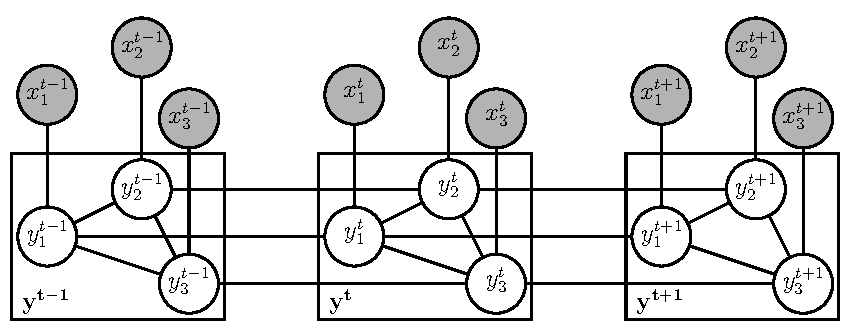
\includegraphics[width=0.5\textwidth]{hmmcrf}
%\vspace{\captionReduceTop}
\caption{The graphical model, we use within the rCRF, is a temporal CRF with additional constraints.}% Shaded nodes represent the observations.
%\vspace{\captionReduceBot}
\label{rCrf}
\end{figure}

\noindent We are interested in the belief over state variables at $t$ as $bel^t(\mathbf{y}) = p(\mathbf{y}^t=\mathbf{y}|\mathbf{x}_1,\ldots,\mathbf{x}_T)$. Following the independence properties, it can be defined as.
\begin{equation}
bel^t(\mathbf{y}) \propto  \underbrace{p(\mathbf{y}^t=\mathbf{y}|\mathbf{x}^1,\ldots,\mathbf{x}^t)}_{\alpha^t(\mathbf{y})} \underbrace{p(\mathbf{x}^{t+1},\ldots,\mathbf{x}^T|\mathbf{y}^t=\mathbf{y})}_{\beta^t(\mathbf{y})}
\label{beldec}
\end{equation}
with recursive definition of $\alpha^t$ and $\beta^t$ as;
\begin{equation}
\begin{aligned}
\alpha^t(\mathbf{y}^t) &= p(\mathbf{x}^t|\mathbf{y}^t)\sum_{\mathbf{y}^{t-1}} \alpha^{t-1}(\mathbf{y}^{t-1}) p(\mathbf{y}^{t}|\mathbf{y}^{t-1}) \\
\beta^t(\mathbf{y}^t) &= \sum_{\mathbf{y}^{t+1}} p(\mathbf{x}^{t+1}|\mathbf{y}^{t+1}) \beta^{t+1}(\mathbf{y}^{t+1}) p(\mathbf{y}^{t+1}|\mathbf{y}^{t})
\end{aligned}
\label{mespas}
\end{equation}
\noindent
with initializations $\alpha^1(\mathbf{y}^1)=p(\mathbf{x}^1|\mathbf{y}^1)$ and $\beta^T(\mathbf{y}^T)=1$.

\subsection{Challanges:}
\begin{itemize}
  \item CRF is modelling $p(\mathbf{y}^t|\mathbf{x}^t)$ instead of $p(\mathbf{x}^t|\mathbf{y}^t)$.
  \item Messages requires a summation over the entire output space which has an exponential dimension.
\end{itemize}

%Finally, we suggest a method to efficiently represent the belief over small number of samples in section \ref{divm}.
\subsubsection{From $p(\mathbf{y}^t|\mathbf{x}^t)$ to $p(\mathbf{x}^t|\mathbf{y}^t)$}
Since $(\mathbf{x}^t,\mathbf{y}^t)$ is a CRF, the posterior of the label given the observation follows; %a Gibbs measure \cite{geman} as;
\begin{equation}
p(\mathbf{y}^t|\mathbf{x}^t) \propto \exp\left( \sum_{i \in V^t} \theta_{x^t_i}(y^t_i) + \sum_{i,j \in E^t} \theta_{x^t_i,x^t_j}(y^t_i,y^t_j)  \right)
\label{crflogl}
\end{equation}
where $\theta$ is the energy function defined over the node set \mbox{$v \in V^t$ }as $\theta_{v}$ and over the edge set \mbox{$(u,v) \in E^t$} as $\theta_{u,v}$.

\begin{equation}
p(\mathbf{y}^t)=\sum_{\mathbf{x}^t} \exp\left( \sum_{i \in V^t} \theta_{x^t_i}(y^t_i) + \sum_{i,j \in E^t} \theta_{x^t_i,x^t_j}(y^t_i,y^t_j) \right) p(\mathbf{x}^t)
\end{equation}
For tractability, we approximate the $p(\mathbf{y}^t)$ with its lower bound after applying the Jensen inequality as;
\begin{equation}
  \small
p(\mathbf{y}^t) \approx \exp ( \sum_{i \in V^t} \underbrace{\sum_{\mathbf{x}^t} \theta_{x^t_i}(y^t_i)  p(\mathbf{x}^t)}_{\tilde{\theta}(y^t_i)} + \sum_{i,j \in E^t} \underbrace{ \sum_{\mathbf{x}^t}  \theta_{x^t_i,x^t_j}(y^t_i,y^t_j) p(\mathbf{x}^t)}_{\tilde{\theta}(y^t_i,y^t_j)} )
\end{equation}

% \todo{
We then estimate the inner summations $\tilde{\theta}(\cdot)$
% , expectation over $\mathbf{x}$, )
% empirically by
% In other words, we
using Monte Carlo
% to compute inner summations
 as \mbox{$\tilde{\theta}(\cdot) = \frac{1}{N}\sum_{i=1}^N \theta_{\mathbf{x}^{(i)}}(\cdot)$} where $\mathbf{x}^{(i)}$ is the $i^{th}$ training sample. The final observation likelihood is:  $p(\mathbf{x}^t|\mathbf{y}^t) \propto$
\begin{equation}\small
\exp\left( \sum_{i \in V^t} \theta_{x^t_i}(y^t_i) - \tilde{\theta}(y^t_i) + \sum_{i,j \in E^t} \theta_{x^t_i,x^t_j}(y^t_i,y^t_j) - \tilde{\theta}(y^t_i,y^t_j)  \right)
\label{obsprob}
\end{equation}

\subsubsection{Belief is a CRF}
\label{beliscrf}
The belief function can be computed as follows:
\begin{equation}\small
  \begin{aligned}
&bel(\mathbf{y}^t) \propto \exp\left[  \sum_{i,j \in E^t} \left( \theta_{x^t_i,x^t_j}(y^t_i,y^t_j) - \tilde{\theta}(y^t_i,y^t_j) \right) \right. \\
&\left. \sum_{i \in V^t} \left( \theta_{x^t_i}(y^t_i) - \tilde{\theta}(y^t_i) +  \sum_{\mathbf{y}^{t-1}} \alpha^{t-1}(\mathbf{y}^{t-1}) \log p(y^t_i|y^{t-1}_i) \right. \right. \\
&+\left.\left.\frac{1}{\gamma}\sum_{\mathbf{y}^{t+1}} \beta^{t+1}(\mathbf{y}^{t+1}) p(\mathbf{x}^{t+1}|\mathbf{y}^{t+1}) \log p(y^{t+1}_i|y^{t}_i) \right) \right]
\end{aligned}
\label{crfbelief}
\end{equation}
This function is graph decomposable hence the posterior belief in rCRF is also a CRF. Hence, we can use the existing learning, inference and structured diversity algorithms developed for CRFs by just modifying the energy functions.
\end{document}
